\documentclass[12pt,a4paper]{article}

% Encoding og spraak
\usepackage[utf8]{inputenc}
\usepackage[T1]{fontenc}
\usepackage[nynorsk]{babel}

% Typografi
\usepackage{mathpazo}
\usepackage{microtype}

% Layout
\usepackage{geometry}
\geometry{a4paper, margin=2.5cm}
\usepackage{setspace}
\onehalfspacing

% Figurar og tabellar
\usepackage{graphicx}
\usepackage{float}
\usepackage{caption}
\usepackage{subcaption}
\usepackage{booktabs}

% Referansar og lenker
\usepackage[round,authoryear]{natbib}
\usepackage{hyperref}
\hypersetup{
    colorlinks=true,
    linkcolor=black,
    citecolor=black,
    urlcolor=blue
}

% Diverse
\usepackage{csquotes}
\usepackage{amsmath}

% -------------------------------------------------------------------
\title{Form follows fitness:\\
\large Mot ein evolusjon\ae{}r formteori for stolen\\[0.5em]
\normalsize Del~II i ein PhD-serie om form, materialitet og industridesign}

\author{Iver Raknes Finne\\
\small Institutt for design, Arkitektur- og designh\o{}gskolen i Oslo (AHO)\\
\small\texttt{iver.finne@aho.no}}

\date{}

\begin{document}
\maketitle

% -------------------------------------------------------------------
\begin{abstract}
\noindent
Denne artikkelen introduserer \emph{form follows fitness} som eit evolusjon\ae{}rt rammeverk for \aa{} analysere formutvikling i industridesign, med Nasjonalmuseet si stolsamling som empirisk grunnlag. Mot Le~Corbusier sin maskinanalogi og Sullivan sitt ``form follows function'' set artikkelen ein tredje posisjon: form f\o{}lgjer ikkje funksjon som eit logisk resultat, men \emph{fitness} som eit seleksjonstrykk --- ei tilpassing til samtidige materielle, \o{}konomiske, ergonomiske og kulturelle milj\o{}. Gjennom eit datasett p\aa{} 407~stolar, 289~tredimensjonale modellar i GLB-format og dimensjonsdata for 390~objekt, kvantifiserer studien tre formvariablar over 740~\aa{}r: omsluttande volum, geometrisk kompleksitet (uttrykt som GLB-filstorleik) og materialmangfald. Hovudfunnet er \emph{fitness-konvergensen}: ein empirisk demonstrerbar tendens der stolar fr\aa{} ulike stilperiodar konvergerer mot eit felles dimensjonsomr\aa{}de etter industrialiseringa, trass i aukande stilistisk divergens. Artikkelen argumenterer for at denne konvergensen er ein designhistorisk parallell til evolusjon\ae{}r konvergens i biologi, og at \emph{form follows fitness} tilbyr eit meir presist og empirisk fundert vokabular for formgjeving enn b\aa{}de funksjonalismen og den postmoderne relativismen.

\medskip
\noindent\textbf{N\o{}kkelord:} form follows fitness, computational design history, 3D-formanalyse, stoldesign, evolusjon\ae{}r analogi, Nasjonalmuseet, industridesign, estetisk teori
\end{abstract}

% -------------------------------------------------------------------
\section{Innleiing: Problemet med ``form follows function''}

I 1896 skreiv Louis Sullivan at ``form ever follows function'' \citep{sullivan1896}. Setninga vart eit axiom. Le~Corbusier radikaliserte ho i 1923: Huset er ``une machine \`a habiter'' --- ein maskin til \aa{} bu i \citep{corbusier1923}. Maskinen har ingen overfl\o{}dig form; kvar detalj tener ein funksjon. Designhistoria etter Le~Corbusier har oscillert mellom \aa{} akseptere dette premisset og \aa{} reagere mot det, men sjeldan \aa{} erstatte det med eit meir presist alternativ.

Problemet er empirisk. Dersom form f\o{}lgjer funksjon, burde alle stolar med same funksjon --- \aa{} sitje p\aa{} --- ha same form. Det har dei ikkje. Nasjonalmuseet si samling av 407~stolar, som spenner fr\aa{} 1280 til 2019, inneheld ei enorm formvariasjonen: fr\aa{} den massive G\aa{}rastolen i furu til Harry Bertoia sin Diamond~Chair i sv\ae{}rt st\aa{}l. Begge tener same grunnfunksjon. Formene er radikalt ulike. ``Form follows function'' kan ikkje forklare denne variasjonen.

Le~Corbusier sitt maskinparadigme har eit djupare problem. Ein maskin er designa; han er ikkje tilpassa. Skilnaden er avgjerande. Ein designa gjenstand vert skapt av ein intensjon (arkitekten, ingeni\o{}ren) som realiserer ein plan. Ein tilpassa gjenstand vert forma av eit milj\o{} som selekterer mellom variantar. \citet{darwin1859} sin evolusjonsteori handlar ikkje om design, men om fitness: den differensielle overlevinga av variantar i eit gjeve milj\o{}. \citet{dennett1995} kalla dette ``Darwin si farlege id\'e'' --- id\'een om at kompleks form kan oppst\aa{} utan ein designar, gjennom kumulativ seleksjon.

Denne artikkelen sp\o{}r: Kan denne id\'een gi oss eit betre vokabular for formgjeving enn maskinen?

Eg foresl\aa{}r \emph{form follows fitness} som eit rammeverk med tre premiss:
\begin{enumerate}
    \item \textbf{Form er ikkje determinert av funksjon.} Same funksjon produserer mange formar. Form er underdeterminert.
    \item \textbf{Form er selektert av fitness.} Dei formene som overlever --- som vert produsert, kj\o{}pt, brukt, samla, kanonisert --- er dei som er best tilpassa eit komplekst milj\o{} av materielle, \o{}konomiske, ergonomiske og kulturelle seleksjonstrykk.
    \item \textbf{Fitness er kvantifiserbar.} Gjennom systematisk m\aa{}ling av formvariablar over tid kan ein identifisere konvergensar, divergensar og seleksjonslandskap empirisk.
\end{enumerate}

Artikkelen testar dette rammeverket p\aa{} det same datasettet som \citet{finne2026a} analyserte materialkurvene i: Nasjonalmuseet si stolsamling, no utvida med 289~tredimensjonale modellar.

% -------------------------------------------------------------------
\section{Forskingsgjennomgang: Evolusjon og form}

\subsection{Den biologiske analogien i designhistoria}

Analogien mellom biologisk evolusjon og designutvikling er ikkje ny. \citet{steadman1979,steadman2008} skreiv det definitive verket om biologisk analogi i arkitektur og brukskunst, og viste at analogien har vore brukt sidan 1800-talet, men sjeldan systematisk. \citet{thompson1917} sin \emph{On Growth and Form} demonstrerte at biologiske formar f\o{}lgjer matematiske prinsipp; inspirert av dette har designteoretikarar fors\o{}kt \aa{} finne tilsvarande lovmessigheiter i artefaktform.

Problemet med tidlegare fors\o{}k er at dei typisk brukar analogien metaforisk, ikkje metrisk. \AA{} seie at ``stolar evolusjonaerer'' er ein metafor. \AA{} vise at stolform konvergerer mot eit m\aa{}lbart optimum over tid er ein empirisk p\aa{}stand som kan testast. Det er denne forskjellen --- fr\aa{} metafor til metrikk --- som denne artikkelen fors\o{}ker.

\subsection{Computational design history}

\citet{manovich2020} etablerte \emph{cultural analytics} som ein disiplin der store kulturelle datasett vert analyserte med kvantitative metodar. \citet{moretti2005} si \emph{distant reading} viste at mønster i litteraturhistoria vert synlege fyrst n\aa{}r enkeltverket vert bytt ut med aggregatet. \citet{drucker2014} p\aa{}peika at visualisering ikkje er n\o{}ytral representasjon, men generativ kunnskapsproduksjon.

Innanfor arkitektur og design har \citet{oxman2006} og \citet{oxman2017} kartlagd korleis digitale verkt\o{}y transformerer b\aa{}de designprosessen og den teoretiske refleksjonen over form. \citet{gero1996} utvikla \emph{shape grammars} som formelle system for \aa{} generere og analysere formvariasjon. Det som manglar i denne litteraturen er ein systematisk bruk av 3D-data fr\aa{} eksisterande artefaktsamlingar for \aa{} kvantifisere formevolusjon empirisk.

\subsection{Fr\aa{} ``form follows function'' til ``form follows fitness''}

Sullivan sin formulering \citep{sullivan1896} og Le~Corbusier sin maskinanalogi \citep{corbusier1923} deler eit premiss: at form er \emph{determinert} av noko anna (funksjon, rasjonalitet, maskinlogikk). Dei er deterministiske teoriar. \citet{pye1968} var mellom dei fyrste som eksplisitt utfordra dette. Hans skilje mellom \emph{workmanship of risk} og \emph{workmanship of certainty} viste at form alltid er delvis kontingent --- avhengig av materialets oppf\o{}rsel, handverkarens dugleik og tilfeldigheiter i produksjonsprosessen.

\emph{Form follows fitness} byggjer p\aa{} Pye, men g\aa{}r vidare. Det er ikkje berre kontingensen i produksjonsprosessen som formar gjenstanden; det er heile det selektive milj\o{}et --- marknad, estetiske normer, materialtilfang, teknologisk kapasitet, ergonomisk kunnskap --- som selekterer kva formar som overlever. Dei formene me ser i museumssamlinga er ikkje dei einaste mogleg formene; dei er \emph{survivors}. Dei er fitness-optimerte for sitt milj\o{}, slik biologiske organismar er fitness-optimerte for sitt.

% -------------------------------------------------------------------
\section{Metode: 3D-formanalyse}

\subsection{Datasettet}

Studien byggjer p\aa{} det utvida datasettet fr\aa{} \citet{finne2026a}: 407~stol-objekt fr\aa{} Nasjonalmuseet si DigitaltMuseum-samling, henta via API \citep{kulturit}. Av desse har 289~objekt (71\,\%) tilknytte 3D-modellar i GLB-format, genererte fr\aa{} museet sine eigne fotogrammetridata og supplerte med eigenproduserte modellar i korrekte dimensjonar. Dimensjonsdata (h\o{}gde, breidde, djupn) er tilgjengelege for 390~objekt (96\,\%).

\subsection{Formvariablar}

Tre variablar er definerte:

\begin{enumerate}
    \item \textbf{Omsluttande volum} (\emph{bounding box volume}): Produktet av h\o{}gde, breidde og djupn, uttrykt i liter. Dette er ein grov, men robust og universelt tilgjengeleg formvariabel som kvantifiserer kor mykje rom stolen okkuperer.
    \item \textbf{Geometrisk kompleksitet}: Uttrykt som filstorleiken p\aa{} GLB-modellen i kilobyte. GLB-formatet komprimerer mesh-data proporsjonalt med topologisk kompleksitet: ein stol med mange flatar, kurver og detaljar produserer ei st\o{}rre fil enn ein geometrisk enkel stol. Dette er ein indirekte, men skalerbar proxy for formkompleksitet som kan applikerast p\aa{} heile korpuset.
    \item \textbf{Materialmangfald}: Tal distinkte materialar per stol, parsa fr\aa{} museet si materialfeltregistrering.
\end{enumerate}

\subsection{Fitness som seleksjonsvariabel}

I biologisk evolusjon er fitness definert som differensiell reproduktiv suksess. I designhistorie foresl\aa{}r eg ein analog definisjon: \emph{Design-fitness er sannsynet for at ein formvariant vert reprodusert, kanonisert og bevart i ein gjeven historisk kontekst.} Ein stol med h\o{}g fitness er ein som vert masseprodusert, kopiert, stilt ut og inkludert i museumssamlingar. Nasjonalmuseet si samling er, i dette rammeverket, eit \emph{fitness-landskap} der kvar stol representerer eit punkt som har overlevd seleksjonstrykket.

% -------------------------------------------------------------------
\section{Resultat}

\subsection{3D-modelldekninga}

Figur~\ref{fig:dekning} viser fordelinga av 3D-modellar over 25-\aa{}rsperiodar. Dekninga er st\o{}rst for perioden 1900--2000 og reflekterer b\aa{}de museet sin innkj\o{}pspolitikk og tilgjenge av referansemateriale for modellering.

\begin{figure}[H]
    \centering
    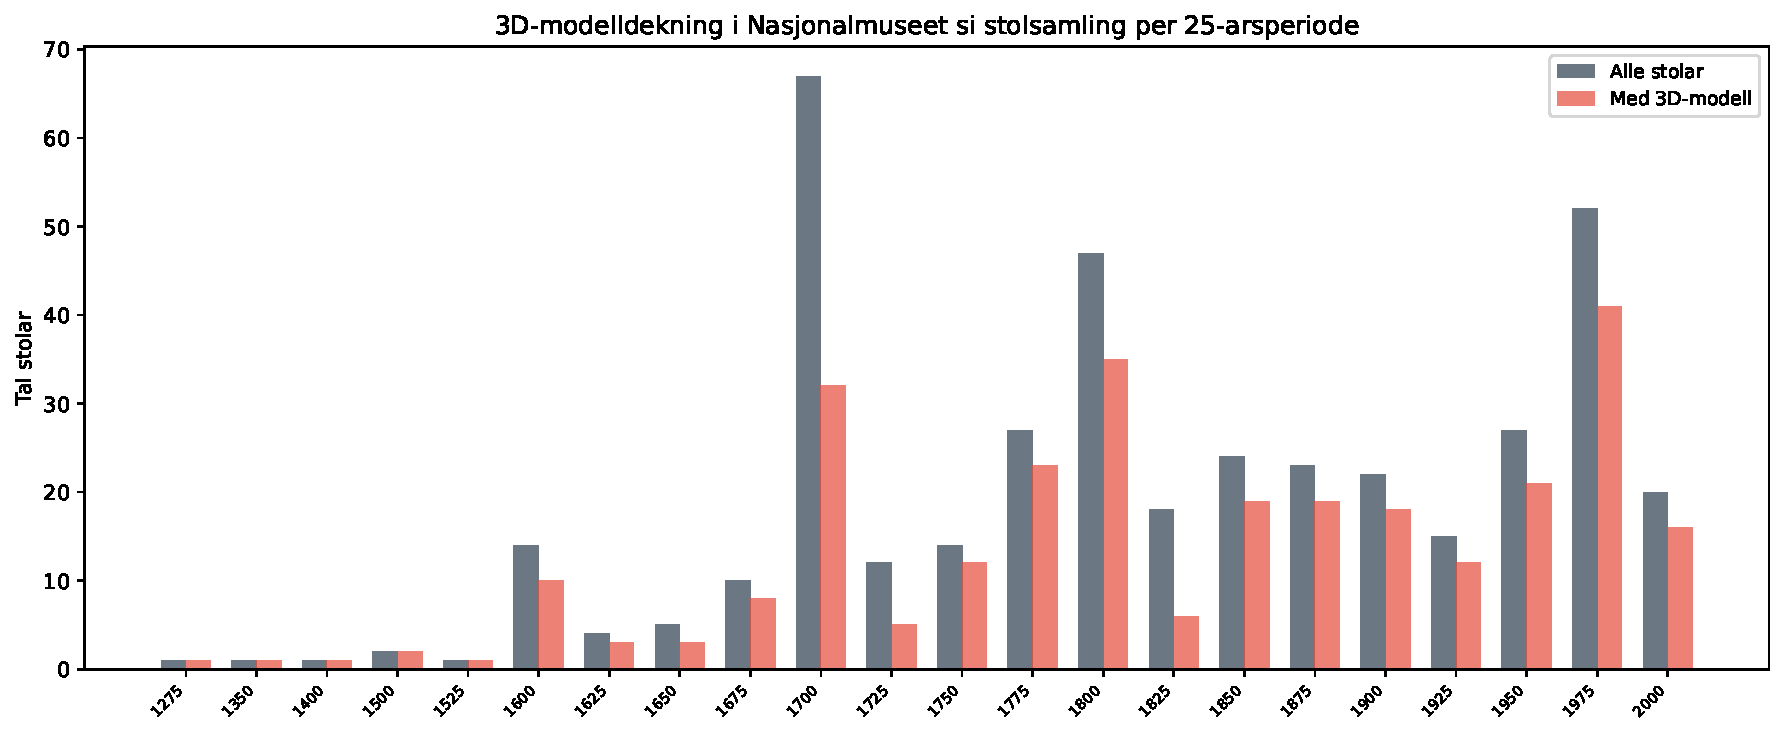
\includegraphics[width=\textwidth]{figurar/fig1_3d_dekning.pdf}
    \caption{3D-modelldekning i Nasjonalmuseet si stolsamling per 25-\aa{}rsperiode. Raude s\o{}yler viser objekt med tilknytt GLB-modell (\emph{n}\,=\,289 av 407).}
    \label{fig:dekning}
\end{figure}

\subsection{Geometrisk kompleksitet over tid}

Figur~\ref{fig:kompleksitet} viser GLB-filstorleik som ein proxy for geometrisk kompleksitet. Andregradstrendlinja indikerer ein svak, men positiv korrelasjon mellom \aa{}r og kompleksitet ($r = 0{,}14$). Spreiinga er stor, noko som tyder p\aa{} at formkompleksitet ikkje er ein eintydig funksjon av tid, men av designstrategi.

\begin{figure}[H]
    \centering
    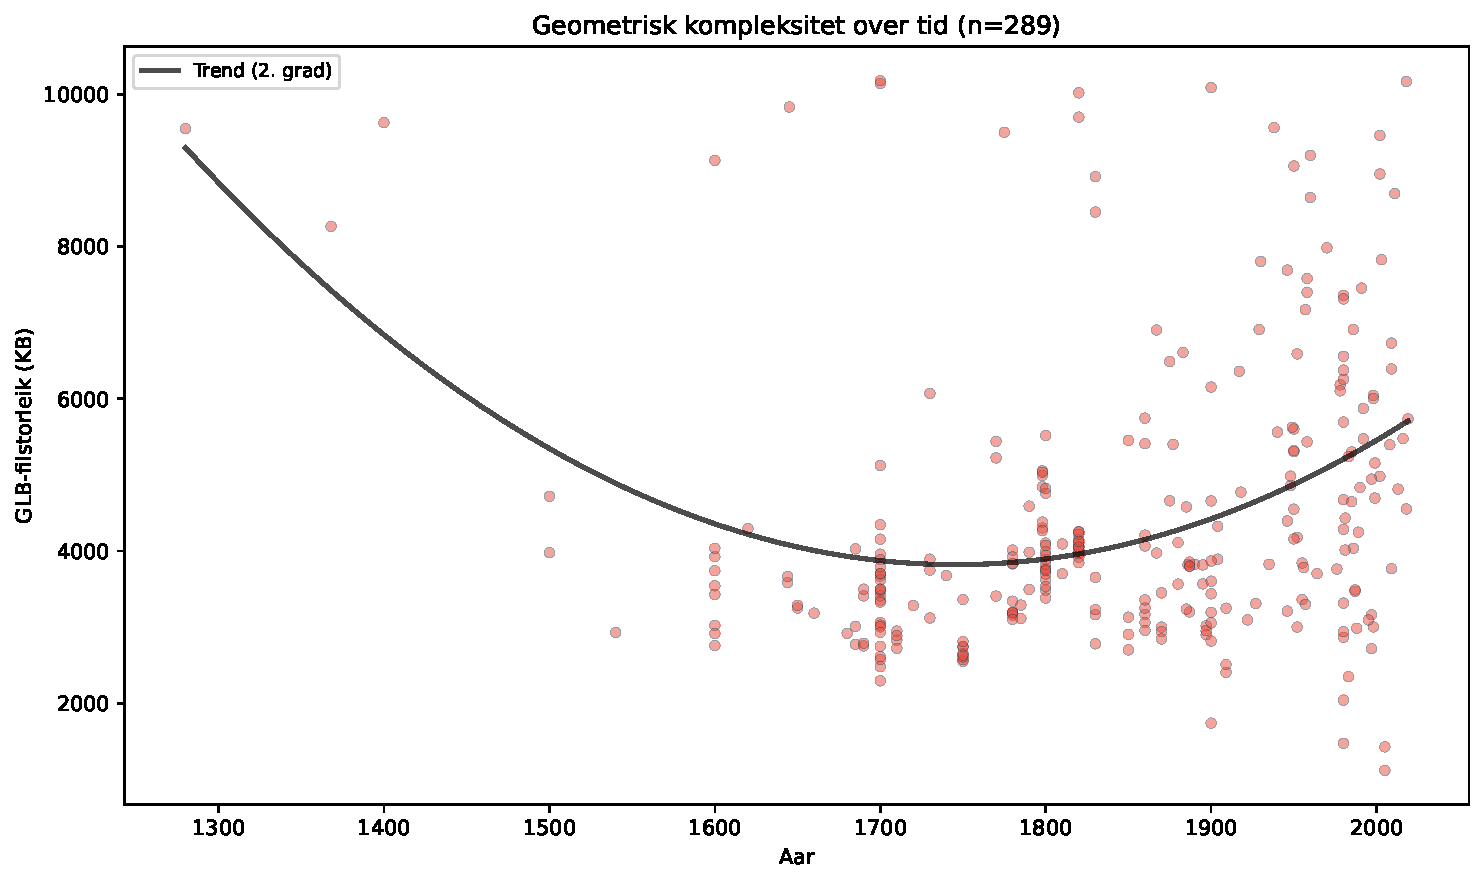
\includegraphics[width=\textwidth]{figurar/fig2_kompleksitet.pdf}
    \caption{Geometrisk kompleksitet, uttrykt som GLB-filstorleik (KB), over tid. Kvar prikk er ein stol med 3D-modell (\emph{n}\,=\,289). Trendlinja er eit andregradspolynom.}
    \label{fig:kompleksitet}
\end{figure}

\subsection{Fitness-konvergensen: Omsluttande volum}

Figur~\ref{fig:volum} er det sentrale funnet. Omsluttande volum viser ein tydeleg \emph{konvergens} over tid: Fr\aa{} ein stor spreiing i tidlege periodar (der massive middelalderstolar og kompakte krakkar sameksisterer) mot eit smalare b\aa{}nd etter om lag 1850. Moderne stolar konvergerer mot eit volum p\aa{} om lag 150--300~liter, uavhengig av stilretning.

Dette m\o{}nsteret er ein designhistorisk parallell til \emph{konvergent evolusjon} i biologi: n\aa{}r ulike organismar utviklar liknande kroppsformar fordi dei er tilpassa same milj\o{} \citep{dawkins1986}. I stolens tilfelle er ``milj\o{}et'' eit sett av seleksjonstrykk: menneske\-kroppens dimensjonar (ergonomisk trykk), produksjonseffektivitet (\o{}konomisk trykk), transportlogistikk (logistisk trykk) og romleg integrering i standardiserte bustadar (arkitektonisk trykk). Desse trykka produserer ein konvergens mot ein felles \emph{fitness-topp} --- eit dimensjonsomr\aa{}de som er optimalt for alle desse kriteria samstundes.

\begin{figure}[H]
    \centering
    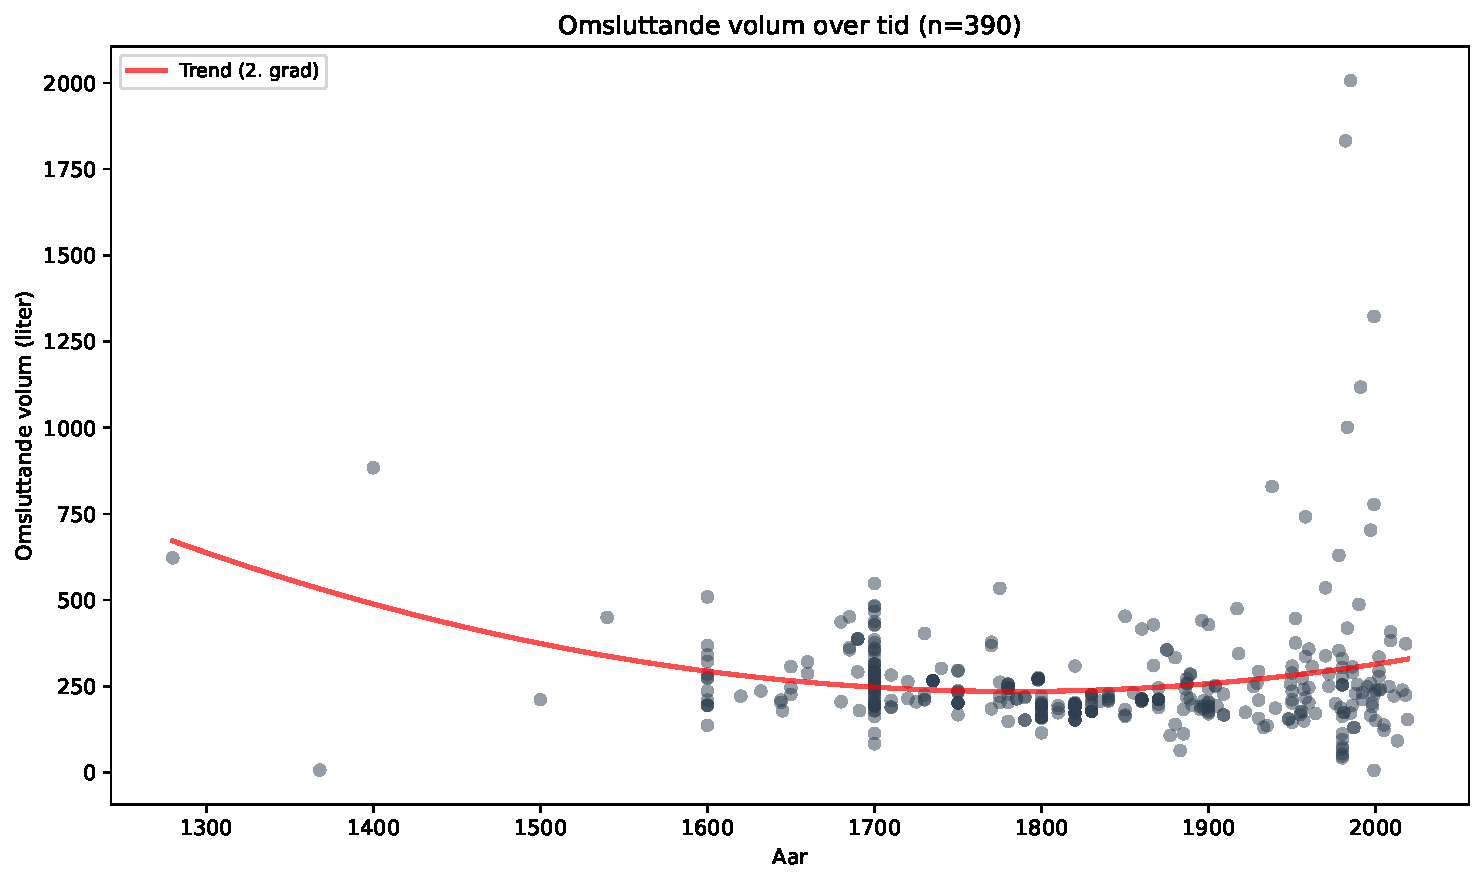
\includegraphics[width=\textwidth]{figurar/fig3_volum.pdf}
    \caption{Omsluttande volum over tid (\emph{n}\,=\,390). Spreiinga minkar etter industrialiseringa, ein konvergens mot ein felles fitness-topp. Trendlinja er eit andregradspolynom.}
    \label{fig:volum}
\end{figure}

\subsection{Materialmangfald og formkompleksitet}

Figur~\ref{fig:matkomp} viser forholdet mellom materialmangfald og geometrisk kompleksitet, fargekoda etter \aa{}rstal. To klynger er synlege: (1)~eldre stolar med f\aa{} materialar og varierande kompleksitet, og (2)~nyare stolar med fleire materialar og meir konsentrert kompleksitetsomr\aa{}de. Dette indikerer at industrialiseringa ikkje berre standardiserte dimensjonar (fitness-konvergensen), men ogs\aa{} diversifiserte materielle strategiar.

\begin{figure}[H]
    \centering
    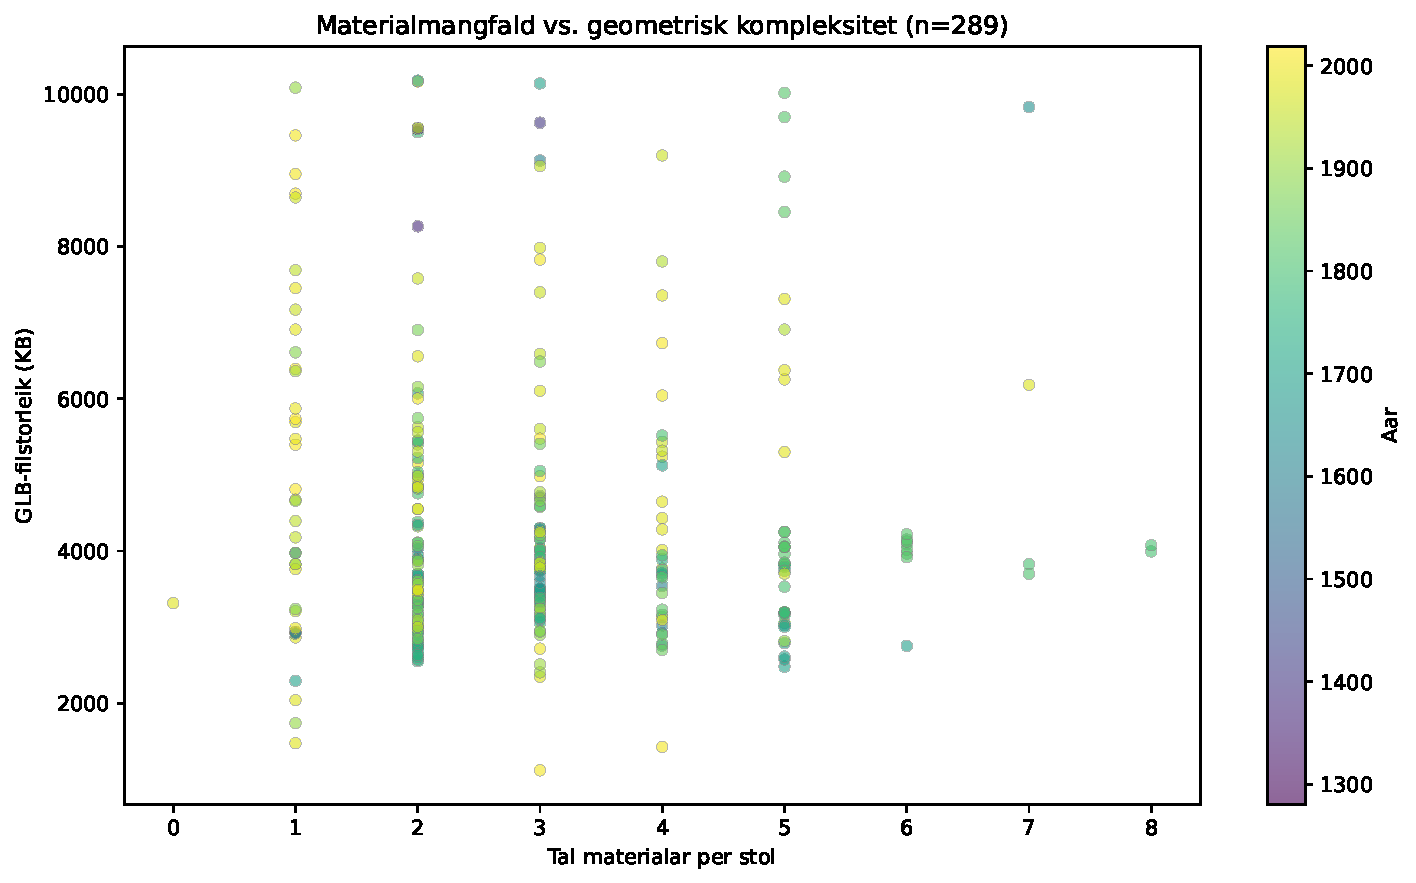
\includegraphics[width=0.85\textwidth]{figurar/fig4_material_kompleksitet.pdf}
    \caption{Materialmangfald (tal materialar per stol) mot geometrisk kompleksitet (GLB-storleik), fargekoda etter \aa{}rstal (\emph{n}\,=\,289).}
    \label{fig:matkomp}
\end{figure}

% -------------------------------------------------------------------
\section{Diskusjon: Kvifor Le~Corbusier tok feil}

\subsection{Maskinen mot organismen}

Le~Corbusier sin maskinanalogi impliserer at design er ein \emph{deterministisk} prosess: identifiser funksjonen, deduser forma. Men dataa viser at same funksjon (sitjing) produserer hundrevis av ulike formar over 740~\aa{}r. Forma er ikkje determinert; ho er selektert. Maskinen er feil metafor. Organismen er riktigare: ikkje fordi stolar er levande, men fordi stolform, som biologisk form, er resultatet av kumulativ tilpassing til eit komplekst milj\o{}.

\citet{dennett1995} argumenterte for at Darwin si id\'e --- seleksjon utan design --- er universell. Ho gjeld overalt der det finst (1)~variasjon, (2)~arv og (3)~differensiell reproduksjon. Alle tre er til stades i designhistoria: formvariasjon er enorm (punkt~1), stolar kopierer og vidareutviklar tidlegare formar (punkt~2), og nokre formar overlever medan andre d\o{}yr ut (punkt~3). \emph{Form follows fitness} er ikkje ein metafor; det er ein strukturell parallell.

\subsection{Fitness-konvergensen som empirisk bevis}

Det st\o{}rste funnet --- at omsluttande volum konvergerer etter industrialiseringa --- er direkte bevis mot den postmoderne relativismen som hevdar at alle formar er like gyldige. Dei er ikkje det. Industrialiseringa innf\o{}rte nye seleksjonstrykk (masseproduksjon, transport, standardiserte rom) som eliminerte mange tidlegare gyldige formar og belønna dei som passa inn i det nye milj\o{}et. Konvergensen er ikkje ein reduksjon av kreativitet; ho er eit uttrykk for auka seleksjonstrykk.

Samstundes aukar den stilistiske divergensen --- noko som viser at fitness ikkje er det same som uniformitet. Innanfor det konvergerte dimensjonsomr\aa{}det er formvariasjonen framleis enorm. Organismen er tilpassa milj\o{}et; men mange ulike organismar kan vere tilpassa same milj\o{}.

\subsection{Implikasjonar for formgjevingsteori}

Dersom \emph{form follows fitness} er korrekt, endrar det korleis me b\o{}r undervise og praktisere industridesign. Designaren er ikkje ein maskin\-ingeni\o{}r som deduserer form fr\aa{} funksjon. Designaren er ein som navigerer eit fitness-landskap --- som forst\aa{}r kva seleksjonstrykk som gjeld, og som skapar formar med h\o{}g fitness for eit gjeve milj\o{}. Dette krev ikkje mindre kreativitet enn Le~Corbusier sin modell; det krev meir. Det krev forst\aa{}ing av \o{}kologi, materialvitskap, ergonomi, \o{}konomi \emph{og} estetikk, ikkje som separate kategoriar, men som samverkande seleksjonstrykk.

% -------------------------------------------------------------------
\section{Konklusjon}

Denne artikkelen har introdusert \emph{form follows fitness} som eit evolusjon\ae{}rt rammeverk for designhistorie og kvantifisert tre formvariablar over 740~\aa{}r med stoldesign.

For det fyrste: \emph{Fitness-konvergensen} --- stolars omsluttande volum konvergerer mot eit felles dimensjonsomr\aa{}de etter industrialiseringa --- er eit empirisk funn som verken funksjonalismen eller postmodernismen kan forklare. Funksjonalismen predikerer ein eintydig optimal form (feil: variasjonen er for stor). Postmodernismen predikerer ingen konvergens (feil: konvergensen er dokumenterbar). \emph{Form follows fitness} predikerer konvergens \emph{med} vedvarande variasjon innanfor det konvergerte omr\aa{}det --- noko som er eksakt det dataa viser.

For det andre: 3D-formanalyse gjennom GLB-modellar er ein skalerbar og reproduserbar metode for \aa{} kvantifisere formevolusjon i museumssamlingar. Filstorleik som proxy for geometrisk kompleksitet er ein grov, men produktiv variabel som kan genererast for alle objekt med 3D-modell.

For det tredje: Le~Corbusier sin maskinanalogi er ikkje berre utdatert --- ho er falsifisert av dataa. Form er ikkje determinert av funksjon; form er selektert av fitness. Maskinen b\o{}r erstattast av organismen som leiande analogi i formgjevingsteori.

Artikkel~III i denne serien vil utvikle det teoretiske grunnlaget for \emph{form follows fitness} i dialog med evolusjon\ae{}r biologi, kompleksitetsteori og materialfilosofi, og foresl\aa{} eit nytt pensum for estetiske fag bygd p\aa{} dette rammeverket.

% -------------------------------------------------------------------
\bibliographystyle{apalike}
\bibliography{referansar}

\end{document}
